\documentclass[11pt,letterpaper]{article}
\usepackage[lmargin=1in,rmargin=1in,tmargin=1in,bmargin=1in]{geometry}
\usepackage{../style/homework}
\usepackage{../style/commands}
\setbool{quotetype}{true} % True: Side; False: Under
\setbool{hideans}{false} % Student: True; Instructor: False

% -------------------
% Content
% -------------------
\begin{document}

\homework{1: Due 09/014}{Blackmail is such an ugly word. I prefer `extortion.' The `x' makes it sound cool.}{Bender Rodriguez, Futurama}

% Problem 1
\problem{10} Showing all your work, find the prime factorizations of the following:
	\begin{enumerate}[(a)]
	\item $45$
	\item $30$
	\item $17$
	\item $44$
	\item $220$
	\end{enumerate} \pspace

\sol
\begin{enumerate}[(a)]
\item $45= 3^2 \cdot 5$
	\[
	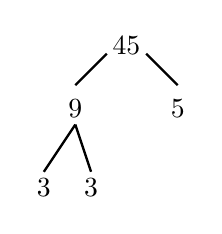
\begin{tikzpicture}
	\node at (-0.15,0) {$45$};
	\draw[line width=0.03cm] (-0.4,-0.1) -- (-0.8,-0.5);
	\node at (-0.8,-0.8) {$9$};
	\draw[line width=0.03cm]  (0.1,-0.1) -- (0.5,-0.5);
	\node at (0.5,-0.8) {$5$};
		
	\draw[line width=0.03cm] (-0.8,-1) -- (-1.2,-1.6);
	\node at (-1.2,-1.8) {$3$};
	\draw[line width=0.03cm] (-0.8,-1) -- (-0.6,-1.6);
	\node at (-0.6,-1.8) {$3$};
	\end{tikzpicture}
	\] \pspace

\item $30= 2 \cdot 3 \cdot 5$
	\[
	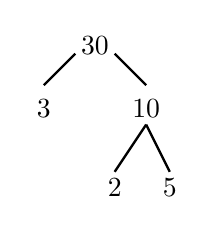
\begin{tikzpicture}
	\node at (-0.15,0) {$30$};
	\draw[line width=0.03cm] (-0.4,-0.1) -- (-0.8,-0.5);
	\node at (-0.8,-0.8) {$3$};
	\draw[line width=0.03cm]  (0.1,-0.1) -- (0.5,-0.5);
	\node at (0.5,-0.8) {$10$};
	
	\draw[line width=0.03cm] (0.5,-1) -- (0.1,-1.6);
	\node at (0.1,-1.8) {$2$};
	\draw[line width=0.03cm] (0.5,-1) -- (0.8,-1.6);
	\node at (0.8,-1.8) {$5$};
	\end{tikzpicture}
	\] \pspace

\item $17= 17^1$

\item $44= 2^2 \cdot 11$
	\[
	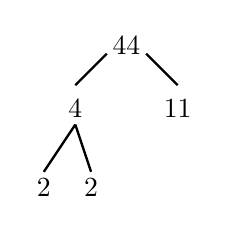
\begin{tikzpicture}
	\node at (-0.15,0) {$44$};
	\draw[line width=0.03cm] (-0.4,-0.1) -- (-0.8,-0.5);
	\node at (-0.8,-0.8) {$4$};
	\draw[line width=0.03cm]  (0.1,-0.1) -- (0.5,-0.5);
	\node at (0.5,-0.8) {$11$};
		
	\draw[line width=0.03cm] (-0.8,-1) -- (-1.2,-1.6);
	\node at (-1.2,-1.8) {$2$};
	\draw[line width=0.03cm] (-0.8,-1) -- (-0.6,-1.6);
	\node at (-0.6,-1.8) {$2$};
	\end{tikzpicture}
	\] \pspace

\item $220= 2^2 \cdot 5 \cdot 11$
	\[
	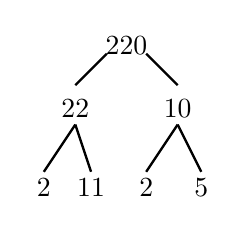
\begin{tikzpicture}
	\node at (-0.15,0) {$220$};
	\draw[line width=0.03cm] (-0.4,-0.1) -- (-0.8,-0.5);
	\node at (-0.8,-0.8) {$22$};
	\draw[line width=0.03cm]  (0.1,-0.1) -- (0.5,-0.5);
	\node at (0.5,-0.8) {$10$};
		
	\draw[line width=0.03cm] (-0.8,-1) -- (-1.2,-1.6);
	\node at (-1.2,-1.8) {$2$};
	\draw[line width=0.03cm] (-0.8,-1) -- (-0.6,-1.6);
	\node at (-0.6,-1.8) {$11$};
	
	\draw[line width=0.03cm] (0.5,-1) -- (0.1,-1.6);
	\node at (0.1,-1.8) {$2$};
	\draw[line width=0.03cm] (0.5,-1) -- (0.8,-1.6);
	\node at (0.8,-1.8) {$5$};
	\end{tikzpicture}
	\] 
\end{enumerate}



\newpage



% Problem 2
\problem{10} Without using a calculator, answer the following:
	\begin{enumerate}[(a)]
	\item Does 2 divide 6701? Explain.
	\item Does 3 divide 3801437? Explain.
	\item Does 4 divide 19154300? Explain.
	\item Does 5 divide 648520? Explain.
	\item Does 9 divide 94321836? Explain. 
	\end{enumerate} \pspace

\sol
\begin{enumerate}[(a)]
\item 2 divides an integer if and only if the integer is even. Because 6701 is not even, 6701 is not divisible by 2. \pspace

\item 3 divides an integer if and only if the sum of its digits is divisible by 3. Because $3 + 8 + 0 + 1 + 4 + 3 + 7= 26$ is not divisible by 3, 3801437 is not divisible by 3. \pspace

\item 4 divides an integer if and only if the last two digits form an integer divisible by 4. Because $00= 0$ is divisible by 4, 19154300 is divisible by 4. \pspace

\item 5 divides an integer if and only if it ends in 0 or 5. Because 648520 ends in 0, 648520 is divisible by 5. \pspace

\item 9 divides an integer if and only if the sum of its digits is divisible by 9. Because $9 + 4 + 3 + 2 + 1 + 8 + 3 + 6= 36$ is divisible by 9, 94321836 is divisible by 9. 
\end{enumerate}



\newpage



% Problem 3
\problem{10} Showing all your work, compute the following:
	\begin{enumerate}[(a)]
	\item $\gcd(10, 14)$
	\item $\lcm(10, 14)$
	\item $\gcd(2^{100} \cdot 3^{40} \cdot 7^{11} \cdot 11^{30},\, 2^{20} \cdot 5^{80} \cdot 7^{60} \cdot 11^{10})$
	\item $\lcm(2^{100} \cdot 3^{40} \cdot 7^{11} \cdot 11^{30},\, 2^{20} \cdot 5^{80} \cdot 7^{60} \cdot 11^{10})$
	\end{enumerate} \pspace

\sol
\begin{enumerate}[(a)]
\item 
	\[
	\gcd(10, 14)= \gcd(2 \cdot 5, 2 \cdot 7)= 2
	\] \pspace

\item 
	\[
	\lcm(10, 14)= \lcm(2 \cdot 5, 2 \cdot 7)= 2 \cdot 5 \cdot 7= 70
	\] \pspace

\item 
	\[
	\gcd(2^{100} \cdot 3^{40} \cdot 7^{11} \cdot 11^{30},\, 2^{20} \cdot 5^{80} \cdot 7^{60} \cdot 11^{10})= 2^{20} \cdot 7^{11} \cdot 11^{10}= 53\,778\,069\,122\,557\,835\,522\,080\,768
	\] \pspace

\item 
	\[
	\lcm(2^{100} \cdot 3^{40} \cdot 7^{11} \cdot 11^{30},\, 2^{20} \cdot 5^{80} \cdot 7^{60} \cdot 11^{10})= 2^{100} \cdot 3^{40} \cdot 5^{80} \cdot 7^{60} \cdot 11^{30}
	\]
\end{enumerate}



\newpage



% Problem 4
\problem{10} Showing all your work and being sure to simplify as much as possible, compute the following:
	\begin{enumerate}[(a)]
	\item $\dfrac{5}{12} - \dfrac{7}{22}$
	\item $\dfrac{3}{4} + \dfrac{7}{8} - \dfrac{1}{6}$
	\item $\dfrac{3}{4} \cdot \dfrac{16}{27} \cdot \dfrac{9}{4}$
	\item $\dfrac{\;\;\dfrac{15}{21}\;\;}{\;\;\dfrac{5}{2}\;\;}$
	\item $\dfrac{\;\;\dfrac{13}{15}\;\;}{\;\;\dfrac{39}{40}\;\;}$
	\end{enumerate} \pspace

\sol
\begin{enumerate}[(a)]
\item
	\[
	\dfrac{5}{12} - \dfrac{7}{22}= \dfrac{55}{132} - \dfrac{42}{132}= \dfrac{13}{132}
	\] \pspace

\item
	\[
	\dfrac{3}{4} + \frac{7}{8} - \frac{1}{6}= \dfrac{18}{24} + \dfrac{21}{24} - \dfrac{4}{24}= \dfrac{35}{24}
	\] \pspace

\item
	\[
	\dfrac{3}{4} \cdot \dfrac{16}{27} \cdot \dfrac{9}{4}= \dfrac{\cancel{3}^{\,1}}{\cancel{4}^{\,1}} \cdot \dfrac{\cancel{16}^{\,\cancel{4}^{\,1}}}{\cancel{27}^{\,\cancel{9}^{\,1}}} \cdot \dfrac{\cancel{9}^{\,1}}{\cancel{4}^{\,1}}= 1
	\] \pspace

\item
	\[
	\dfrac{\;\;\dfrac{15}{21}\;\;}{\;\;\dfrac{5}{2}\;\;}= \dfrac{15}{21} \cdot \dfrac{2}{5}= \dfrac{\cancel{15}^{\,\cancel{3}^{\,1}}}{\cancel{21}^{\,7}} \cdot \dfrac{2}{\cancel{5}^{\,1}}= \dfrac{2}{7}
	\] \pspace

\item
	\[
	\dfrac{\;\;\dfrac{13}{15}\;\;}{\;\;\dfrac{39}{40}\;\;}= \dfrac{13}{15} \cdot \dfrac{40}{39}= \dfrac{\cancel{13}^{\,1}}{\cancel{15}^{\,3}} \cdot \dfrac{\cancel{40}^{\,8}}{\cancel{39}^{\,3}}= \dfrac{8}{9}
	\]
\end{enumerate}



\newpage



% Problem 5
\problem{10} For each of the following, either convert the given improper fraction to a mixed number or the given mixed number to an improper fraction:
	\begin{enumerate}[(a)]
	\item $5 \frac{7}{8}$
	\item $\frac{90}{7}$
	\item $\frac{27}{5}$
	\item $-6 \frac{3}{4}$
	\end{enumerate} \pspace

\sol
\begin{enumerate}[(a)]
\item 
	\[
	5 \frac{7}{8}= \dfrac{5(8) + 7}{8}= \dfrac{40 + 7}{8}= \dfrac{47}{8}
	\] \pspace

\item 
	\[
	\dfrac{90}{7}= \dfrac{84 + 6}{7}= \dfrac{12(7) + 6}{7}= 12 \tfrac{6}{7}
	\] \pspace

\item 
	\[
	\dfrac{27}{5}= \dfrac{25 + 2}{5}= \dfrac{5(5) + 2}{5}= 5 \tfrac{2}{5}
	\] \pspace

\item 
	\[
	-6 \frac{3}{4}= - \left( 6 \frac{3}{4} \right)= -\left( \dfrac{6(4) + 3}{4} \right)= -\left( \dfrac{24 + 3}{4} \right)= -\dfrac{27}{4}
	\]
\end{enumerate}



\newpage



% Problem 6
\problem{10} For each of the following, either convert the given fraction to a decimal or the given decimal to a fraction:
	\begin{enumerate}[(a)]
	\item $\frac{3}{8}$
	\item $0.35$
	\item $\frac{30}{7}$
	\item $0.\overline{75}$
	\end{enumerate} 

\sol
\begin{enumerate}[(a)]
\item 
	\[
	\longdivision{3}{8}
	\] 
	\[
	\dfrac{3}{8}= 0.375
	\]

\item 
	\[
	0.35= \dfrac{35}{100}= \dfrac{\cancel{35}^{\,7}}{\cancel{100}^{\,20}}= \dfrac{7}{20}
	\]

\item 
	\[
	\longdivision{30}{7}
	\] 
	\[
	\dfrac{30}{7}= 4.\overline{285714}
	\]



\newpage



\item \phantom{.}\par
	\begin{table}[!ht]
	\centering\small
	\begin{tabular}{rccc}
	& $100N$ & $=$ & $75.7575757575\overline{75}$ \\ 
	$-$ & $N$ & $=$ & $\phantom{0}0.7575757575\overline{75}$ \\ \hline
	& $99N$ & $=$ & $75$ \\[0.1cm]
	& $N$ & $=$ & $\frac{75}{99}$ \\[0.1cm]
	& $N$ & $=$ & $\frac{25}{33}$
	\end{tabular}
	\end{table} \par
\end{enumerate}







\end{document}